\documentclass[12pt, twoside]{report}

\usepackage{multicol}
\usepackage{amsmath}

%% comment this line for handouts. Uncomment for lecture notes
%\newcommand{\lectureNoteMode}{}

\raggedbottom

\usepackage{color, xifthen, amsthm, amssymb, amsmath, tikz, pgfplots}
\pgfplotsset{compat=1.18}
\usetikzlibrary{backgrounds}
\usepackage[letterpaper, margin=1in]{geometry}
\usepackage{multicol}
\usepackage{fourier}  %don't use txfonts b/c the sf doesn't look good

\usepackage{enumitem}
\setlist{topsep=-\parskip/2}


\setlength{\parindent}{0pt}
\setlength{\parskip}{\baselineskip}


\usepackage{mdframed} % makes better frames around examples (eg pagebreak allowed)
  % from mdframed package. used for examples
\newmdenv[
  skipabove=10pt,%\topsep,
  skipbelow=10pt,%\topsep
  ]{allrules}

\usepackage{tcolorbox} % for colored boxes


\usepackage{subfigure}
\usepackage{hyperref}
\hypersetup{colorlinks, urlcolor=red, linkcolor=.} %color urls, but not interal refs
\usepackage{graphicx, floatflt}
\graphicspath{{./figs/}{../figs/}}
\DeclareGraphicsExtensions{.png,.jpg,.pdf}

\usepackage{wrapfig}  %useful for wrapping text around pictures or tables
		      %though it doesn't do a great job inside my example boxes


\definecolor{defbod}{rgb}{.8,.8,.8}     \definecolor{defhead}{rgb}{.7,.1,.1}
\definecolor{thmbod}{rgb}{.8,.8,.8}     \definecolor{thmhead}{rgb}{.1,.1,.9}
\definecolor{factbod}{rgb}{1,1,1}    \definecolor{facthead}{rgb}{.1,.7,.1}
\definecolor{exbod}{rgb}{1,1,1}         \definecolor{exhead}{rgb}{0,.3,0}
\definecolor{soltext}{rgb}{.2,.2,.5}
\definecolor{notebod}{rgb}{.9,.9,.9}    \definecolor{notehead}{rgb}{.1,.1,.7}

\newcommand{\defn}[1]{
 \noindent \colorbox{defbod}{\begin{minipage}{.95\linewidth}
 \hspace{-12pt}\colorbox{defhead}{\sf\color{white} Definition}
 #1
 \end{minipage} } \medskip
 }
\newcommand{\dt}[1]{\textcolor{defhead}{\bfseries #1}}

\newcommand{\thrm}[1]{
 \noindent \colorbox{thmbod}{\begin{minipage}{.95\linewidth}
 \hspace{-12pt}\colorbox{thmhead}{\sf\color{white}Theorem}
 #1
 \end{minipage} } \medskip
 }
\newcommand{\coro}[1]{
 \noindent \colorbox{thmbod}{\begin{minipage}{.95\linewidth}
 \hspace{-12pt}\colorbox{thmhead}{\sf\color{white}Corollary}
 #1
 \end{minipage} } \medskip
 }
\newcommand{\fact}[1]{  %%%% !! note this different from calcnotes
 \noindent \begin{allrules}
 #1
 \end{allrules} \medskip
 }

\newcommand{\note}[1]{
	\noindent \colorbox{notebod}{\begin{minipage}{.95\textwidth}
			\hspace{-12pt}\colorbox{notehead}{\sf\color{white}NOTE}
			#1
	\end{minipage} } \medskip
}


% making the example thing with a line down the left.
\newmdenv[
rightline=false,
bottomline=false,
skipabove=0pt,%\topsep,
skipbelow=0pt,%\topsep
]{siderules}

\newcommand{\ex}[1]{
  \noindent \begin{siderules}
    \textcolor{exhead}{\sf Example}
    #1
  \end{siderules} 
  \medskip
}




%%%%%%%%%% set it up so that these are not displayed when 
%%%%%%%%%% printing notes for students?  or for overhead?
\newcommand{\exsol}[1]{
  {\color{soltext} #1}
}

\newcommand{\mynonumsect}[2][]{
 \cleardoublepage
 \section*{#1\hskip16pt #2}
 \addcontentsline{toc}{section}{#1 #2}
}

\newcommand{\myhead}[1]{
\par%\vskip\baselineskip
\noindent
{\large\bf #1}
}

%%%%%%%%%%%%%%%%%%%%%%%%
% symbol shortcuts

\newcommand{\nice}{\displaystyle}
\newcommand{\eqq}{\ensuremath \stackrel{?}{=}}
\newcommand{\R}{\ensuremath{\mathbb{R}}}




% %%%%%%%%%%%%%%%%%%%%%%%%
% %
% % Creating handouts vs notes
% %% If you use the line below before loading this file then it will be set up for
% %% lecture notes.  Default is for handouts
% %%
% %% \newcommand{\lectureNoteMode}{}
% %%
% %% do not uncomment here, just add the line to the file where you input this one.
% \ifthenelse{\not\isundefined\lectureNoteMode}
% { % lecture notes 
%   \newcommand{\Hvskip}[1]{}
%   \newcommand{\Hvfill}{}
%   \newcommand{\Hpbreak}{}  % pagebreaks for handouts
%   \newcommand{\Npbreak}{\vfill\pagebreak} % pagebreaks for printable notes
%   \newcommand{\Nonly}[1]{#1} % shows in notes, not in handouts
%   \newcommand{\mycleardoublepage}{\cleardoublepage}

%   \newcommand{\ex}[1]{
%    \noindent \begin{allrules}
%     \textcolor{exhead}{\sf Example}\par
%     #1
%     \end{allrules} \medskip
%   }

% } 
% { 
% %% Handout mode 
% %% this section sets it up with smaller margins, and blank spots for writing solns to examples
%   %%%%%%%%%%%%%%%%%%%%%%%%%%%%%%%%%%%%%%%%%%
%   %change frame around examples
%   % from mdframed package
%   \newmdenv[
%   rightline=false,
%   bottomline=false,
%   skipabove=0pt,%\topsep,
%   skipbelow=0pt,%\topsep
%   ]{siderules}
  
%   \newcommand{\ex}[1]{
%     \noindent \begin{siderules}
%       \textcolor{exhead}{\sf Example}
%       #1
%     \end{siderules} 
%     \medskip
%   }
  
%   %
%   %%%%%%%%%%%%%%%%%%%%%%%%%%%%%%%%%%%%%%%%%%
  
%   % don't show solutions for examples
%   \renewcommand{\exsol}[1]{}
  
%   %used for making blank space in handouts. eg: \vs2
%   \newcommand{\Hvskip}[1]{\vskip#1in\null}
%   \newcommand{\Hvfill}{\vfill} %vfill only in handouts mode
%   \newcommand{\Hpbreak}{\pagebreak} % pagebreaks for handouts
%   \newcommand{\Npbreak}{} % pagebreaks for printable notes
%   \newcommand{\Nonly}[1]{} % shows in printable, not in handouts
%   \newcommand{\mycleardoublepage}{\newpage} % don't need blank pages if not printing
  
%   % don't really need margins since not printing.
%   \geometry{margin=0.75in}

%   \renewcommand{\mynonumsect}[2][]{
%     \mycleardoublepage
%     \section*{#1\hskip16pt Handout: #2}
%     \addcontentsline{toc}{section}{#1 #2}
%   }

% } 





\setlength{\parindent}{0pt}

\setcounter{chapter}{1}
\begin{document}


\mynonumsect[1.2]{Domain and Range}

\textbf{Goal:} To determine the domain and range of functions and their graphs


\defn{The \dt{Domain} of a function is the set of all possible input values.  \\
	The \dt{Range} of a function is the set of all possible output values.}

\myhead{Notation}

\defn{
\dt{Interval Notation:}
	We can describe the domain and range of a function using intervals of values, referred to by the starting and ending values.  
	\begin{itemize}
		\item Curved parentheses are used for “strictly less than.” \\
		 A parenthesis, ) or (, is used if the endpoint is not included.
	
		\item Square brackets are used for “less than or equal to.”  \\
		A bracket, {]} or {[}, is used if the endpoint is included.
		
		\item Since infinity is not a number, we can’t include it in the interval, so we always use curved parentheses with $\infty$ and $\-infty$.
		
		\item 	We use the union symbol, $\cup$ , to combine two unconnected intervals together.  
	\end{itemize}
}


\ex{ Fill in the missing spaces with the other notation.


\begin{center}
	\begin{tabular}{|c|c|p{3in}|}
		\hline
		\textbf{Inequality} & \textbf{Interval Notation} & \textbf{Line Graph} \\
		\hline
		& & \\
		$x > 3$ &  & \\
		& & \\
		\hline
		& & \\
		$t \leq 7$ &  & \\
		& & \\
		\hline
		& & \\
		$-3 < x \leq 5$ &  & \\
		& & \\
		\hline
		& & \\
		& $[1, 15]$ & \\
		& & \\
		\hline
		& & \\
		& $(-\infty, 3)$ & \\
		& & \\
		\hline
		& & \\
		$1\leq x \leq 3$ or $x>5$ & & \\
		& & \\
		\hline
	\end{tabular}
\end{center}
}


\pagebreak 




\myhead{Domain and Range from Graphs}

We can also talk about domain and range based on graphs.  
\begin{itemize}
	\item Since domain refers to the set of possible input values, the domain of a graph consists of all the input values shown on the graph.  Remember that input values are almost always shown along the horizontal axis of the graph. 
	\item  Likewise, since range is the set of possible output values, the range of a graph we can see from the possible values along the vertical axis of the graph.  
	\item Be careful – if the graph continues beyond the window on which we can see the graph, the domain and range might be larger than the values we can see.
\end{itemize}


\ex{Determine the domain and range of each graph below.}
	
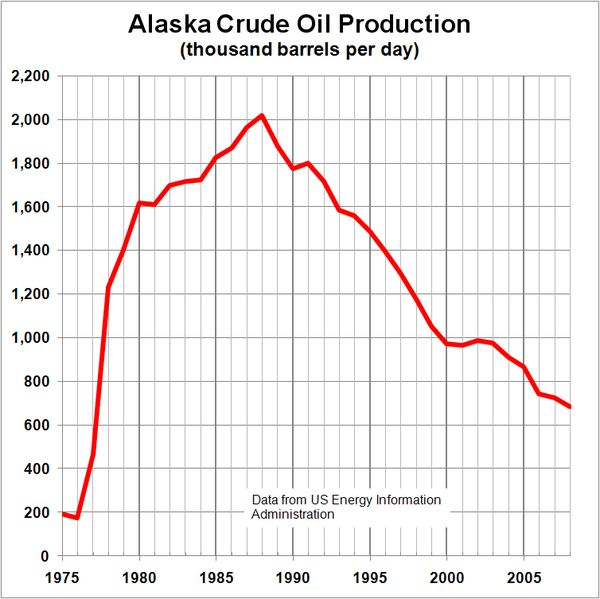
\includegraphics[alt={Graph of Alaska crude oil production over time, used to identify the domain and range from a real-world graph.}, width=3.5in]{105_1.2_figure1.jpg} \hfill
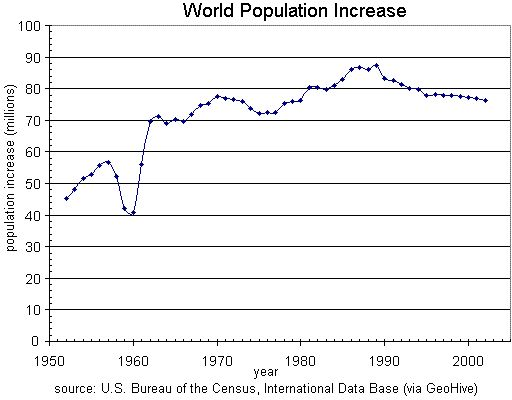
\includegraphics[alt={Graph of world population over time, used to identify the domain and range from a real-world graph.}, width=3.5in]{105_1.2_figure2.jpg} \\
\small{
	\href{https://commons.wikimedia.org/wiki/File:Alaska_Crude_Oil_Production.PNG}{source: wikimedia}
}

\vskip0.25in 

\begin{tabular}{|l|p{3in}|p{3in}|}
	\hline
	& Alaska Crude Oil & World Population \\
	\hline 
	&& \\
	&& \\
	Domain & & \\
	&& \\
	&& \\
	\hline
	&& \\
	&& \\
	Range & & \\ 
	&& \\
	&& \\
	\hline 
\end{tabular}




\pagebreak


\myhead{Domain and Range from Formulas}


\note{\dt{Finding Domain Algebraically}
	
When determining the domain algebraically from formulas, we need to remember these two rules: \\
\begin{itemize}
  \item We cannot divide by 0
  \item We cannot take the square root of a negative number
\end{itemize}
}


\begin{enumerate}
	\item Find the domain of the function \(f(x) = \dfrac{1}{x}\).
 	\vfill
  
	\item Find the domain of the function $f(x)=\dfrac{7}{2x+3}$. 
	\vfill
  
	\item Find the domain of the function $f(x)=\sqrt{4x-5}$. 
	\vfill 
\end{enumerate}


\pagebreak




\myhead{Piecewise Functions}

Some functions cannot be described by a single formula.  

\defn{A \dt{Piecewise function} is a function in which the formula used depends upon the domain the input lies in.  We notate this idea like:

\begin{center}
	$
	f(x) = 
	\begin{cases}
		\text{formula1} & \text{if domain to use formula1} \\
		\text{formula2} & \text{if domain to use formula2} \\
		\text{formula3} & \text{if domain to use formula3} 
	\end{cases}
	$
\end{center}

}



\ex{A museum charges $\$5$ per person for a guided tour with a group of 1 to 9 people, or a fixed $\$50$ fee for 10 or more people in the group.  Set up a function relating the number of people, n, to the cost, C.
}
\vfill 


\ex{A cell phone company uses the function below to determine the cost, $C$, in dollars for $g$ gigabytes of data transfer.  

$C(g)=
\begin{cases}
	25 & \text{if \hskip0.25in} 0<g<2 \\
	25+10(g-2) & \text{if \hskip0.25in} g \geq 2
\end{cases}
$

Find the cost of using 1.5 gigabytes of data, and the cost of using 4 gigabytes of data.
}	
\vfill 


\end{document}
